% SPDX-License-Identifier: CC-BY-NC-ND-4.0

\section{$\lambda$計算}

\begin{definition}
$V$を可算集合とし$V$の元を\textbf{変数}(variable)と呼ぶことにする.\ $\Lambda$を次の条件を満たす最小の集合とする.
\begin{itemize}
    \item $V \subset \Lambda$
    \item ${^{\forall}}M, N \in \Lambda, (M N) \in \Lambda$
    \item ${^{\forall}}x \in V, {^{\forall}}M \in \Lambda, (\lambda x.M) \in \Lambda$
\end{itemize}
$\Lambda$の元を\textbf{$\lambda$項}($\lambda$-term)と呼ぶ.
\end{definition}

BNF記法を用いて$\lambda$項$e$は次のように定義できる.\ ただし$x$は変数である.
\begin{center}
$e ::= x \mid \lambda x. e \mid e e$
\end{center}

\begin{center}
\definecolor{sdgLine}{RGB}{57,70,86}
\definecolor{sdgTermFill}{RGB}{238,243,251}
\definecolor{sdgTermLine}{RGB}{58,103,168}
\definecolor{sdgSpecFill}{RGB}{255,246,230}
\definecolor{sdgSpecLine}{RGB}{184,134,11}
\definecolor{sdgExcFill}{RGB}{253,236,235}
\definecolor{sdgExcLine}{RGB}{176,65,58}
\definecolor{sdgLabel}{RGB}{106,118,134}
\adjustbox{max size={\linewidth}{\textheight}}{%
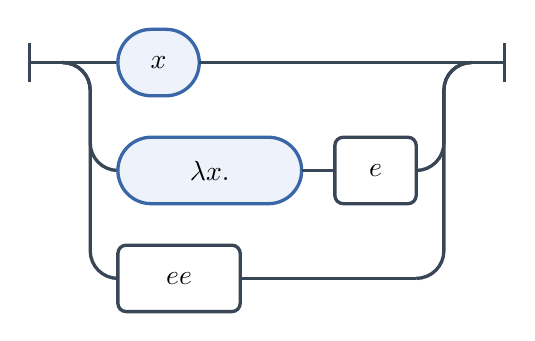
\begin{tikzpicture}[x=1pt, y=1pt]
  \draw[line width=1.2pt, draw=sdgLine, rounded corners=10pt] (8,105) -- (8,91);
  \draw[line width=1.2pt, draw=sdgLine, rounded corners=10pt] (8,98) -- (20,98);
  \draw[line width=1.2pt, draw=sdgLine, rounded corners=10pt] (20,98) -- (40,98);
  \draw[line width=1.2pt, draw=sdgTermLine, fill=sdgTermFill, rounded corners=12pt] (40,86) rectangle (69.4,110);
  \node at (54.7,98) {$x$};
  \draw[line width=1.2pt, draw=sdgLine, rounded corners=10pt] (69.4,98) -- (147.8,98);
  \draw[line width=1.2pt, draw=sdgLine, rounded corners=10pt] (147.8,98) -- (167.8,98);
  \draw[line width=1.2pt, draw=sdgLine, rounded corners=10pt] (20,98) -- (30,98) -- (30,59) -- (40,59);
  \draw[line width=1.2pt, draw=sdgTermLine, fill=sdgTermFill, rounded corners=12pt] (40,47) rectangle (106.4,71);
  \node at (73.2,59) {$\lambda x.$};
  \draw[line width=1.2pt, draw=sdgLine, rounded corners=10pt] (106.4,59) -- (118.4,59);
  \draw[line width=1.2pt, draw=sdgLine, fill=white, rounded corners=3pt] (118.4,47) rectangle (147.8,71);
  \node at (133.1,59) {$e$};
  \draw[line width=1.2pt, draw=sdgLine, rounded corners=10pt] (147.8,59) -- (157.8,59) -- (157.8,98) -- (167.8,98);
  \draw[line width=1.2pt, draw=sdgLine, rounded corners=10pt] (20,98) -- (30,98) -- (30,20) -- (40,20);
  \draw[line width=1.2pt, draw=sdgLine, fill=white, rounded corners=3pt] (40,8) rectangle (84.2,32);
  \node at (62.1,20) {$e e$};
  \draw[line width=1.2pt, draw=sdgLine, rounded corners=10pt] (84.2,20) -- (147.8,20);
  \draw[line width=1.2pt, draw=sdgLine, rounded corners=10pt] (147.8,20) -- (157.8,20) -- (157.8,98) -- (167.8,98);
  \draw[line width=1.2pt, draw=sdgLine, rounded corners=10pt] (167.8,98) -- (179.8,98);
  \draw[line width=1.2pt, draw=sdgLine, rounded corners=10pt] (179.8,105) -- (179.8,91);
\end{tikzpicture}%
}
\end{center}

\begin{remark}
$M,N,P \in \Lambda$に対して$((M N) P)$を$M N P$と表記し$(\lambda x.(\lambda y.M))$を$\lambda x. \lambda y.M$と表記する.
\end{remark}

\begin{definition}
$M \in \Lambda$の自由変数全体の集合$\textrm{FV}(M)$を次のようにして帰納的に定める.
\begin{itemize}
    \item ${^{\forall}}x \in V, \textrm{FV}(x) = \{x\}$
    \item ${^{\forall}}M, N \in \Lambda, \textrm{FV}(M N) = \textrm{FV}(M) \cup \textrm{FV}(N)$
    \item ${^{\forall}}x \in V, {^{\forall}}M \in \Lambda, \textrm{FV}(\lambda x.M) = \textrm{FV}(M) \setminus \{x\}$
\end{itemize}
\end{definition}

\begin{definition}
$M \in \Lambda$の変数全体の集合$\textrm{Var}(M)$を次のようにして帰納的に定める.
\begin{itemize}
    \item ${^{\forall}}x \in V, \textrm{Var}(x) = \{x\}$
    \item ${^{\forall}}M, N \in \Lambda, \textrm{Var}(M N) = \textrm{Var}(M) \cup \textrm{Var}(N)$
    \item ${^{\forall}}x \in V, {^{\forall}}M \in \Lambda, \textrm{Var}(\lambda x.M) = \textrm{Var}(M) \cup \{x\}$
\end{itemize}
\end{definition}

\begin{definition}
$M, N \in \Lambda$に対して$M \lbrack x \coloneq N \rbrack \in \Lambda$を次のようにして帰納的に定める.
\begin{itemize}
    \item ${^{\forall}}x \in V, x \lbrack x \coloneq N \rbrack \equiv N$
    \item ${^{\forall}}x,y \in V, x \neq y \implies y \lbrack x \coloneq N \rbrack \equiv y$
    \item ${^{\forall}}P,Q \in \Lambda, (PQ) \lbrack x \coloneq N \rbrack \equiv (P \lbrack x \coloneq N \rbrack)(Q \lbrack x \coloneq N \rbrack)$
    \item ${^{\forall}}P \in \Lambda, (\lambda x.P) \lbrack x \coloneq N \rbrack \equiv \lambda y.(P \lbrack x \coloneq N \rbrack)$
\end{itemize}
\end{definition}

\begin{definition}
$M \in \Lambda$とし$x, z \in V, y \notin \textrm{Var}(M)$とする.\ $M \langle x \mapsto y\rangle$を次のようにして帰納的に定める.
\begin{itemize}
    \item $x \langle x \mapsto y \rangle \equiv y$
    \item $x \not\equiv z \implies z \langle x \mapsto y \rangle \equiv z$
    \item ${^{\forall}} P, Q \in \Lambda, (PQ) \langle x \mapsto y \rangle \equiv (P \langle x \mapsto y \rangle)(Q \langle x \mapsto y \rangle)$
    \item $z\not\equiv x \implies (\lambda z.P)\langle x \mapsto y\rangle \equiv \lambda z.\big(P\langle x \mapsto y\rangle\big)$
\end{itemize}
\end{definition}

\begin{definition}
$\Lambda$上の2項関係$\to_\alpha \subset \Lambda \times \Lambda$を次のようにして定める.
\begin{center}
    $\to_\alpha \coloneq \{(\lambda x.M, \lambda y.(M \langle x \mapsto y\rangle)) \mid x,y \in V, M \in \Lambda, y \notin \textrm{Ver}(M)\}$
\end{center}
$\to_\alpha$を\textbf{$\alpha$ステップ}($\alpha$-step)と呼ぶ.\ つまり$x,y \in V, M \in \Lambda, y \notin \textrm{Ver}(M)$に対して
\begin{center}
    $\lambda x.M \to_\alpha \lambda y.(M \langle x \mapsto y\rangle)$
\end{center}
である.
\end{definition}

\begin{definition}
$\equiv_\alpha \subset \Lambda \times \Lambda$を次の条件を満たす最小の$\lambda$上の2項関係とする.
\begin{itemize}
    \item $\to_\alpha \subset \equiv_\alpha$
    \item $\equiv_\alpha$は同値関係
    \item ${^{\forall}}z \in V, {^{\forall}}M,M',N \in \Lambda, (M \equiv_\alpha M' \implies (M N \equiv_\alpha M' N) \land (N M \equiv_\alpha N M') \land (\lambda z.M \equiv_\alpha \lambda z.M'))$
\end{itemize}
$\equiv_\alpha$を\textbf{$\alpha$変換}($\alpha$-conversion)という.
\end{definition}

\begin{example}
$\lambda x.\lambda y.x \equiv_\alpha \lambda y.\lambda x.y$
\end{example}

\begin{definition}
$\Lambda$上の2項関係$\to_\beta \subset \Lambda \times \Lambda$を次のようにして定める.
\begin{center}
    $\to_\beta \coloneq \{((\lambda x.M)N, M \lbrack x \coloneq N \rbrack) \mid x \in V, M, N \in \Lambda\}$
\end{center}
$\to_\beta$を\textbf{1ステップ$\beta$簡約}(one-step $\beta$-reduction)という.
\end{definition}

\begin{definition}
$\twoheadrightarrow_\beta \subset \Lambda \times \Lambda$を次の条件を満たす最小の$\lambda$上の2項関係とする.
\begin{itemize}
    \item $\to_\beta \subset \twoheadrightarrow_\beta$
    \item $\twoheadleftarrow$は反射的かつ推移的.
\end{itemize}

$\twoheadrightarrow_\beta$を\textbf{$\beta$簡約}($\beta$-reduction)という.
\end{definition}

\begin{definition}
$=_\beta \subset \Lambda \times \Lambda$を次の条件を満たす最小の$\lambda$上の2項関係とする.
\begin{itemize}
    \item $\to_\beta \subset =_\beta$
    \item $=_\beta$は同値関係.
\end{itemize}
$=_\beta$を\textbf{$\beta$変換}($\beta$-conversion)という.
\end{definition}

\begin{theorem} (Church-Rosser)
\begin{center}
${^{\forall}}M, N_1, N_2 \in \Lambda, ((M \twoheadrightarrow_\beta N_1 \land M \twoheadrightarrow_\beta N_2) \implies ({^{\exists}}N_3 \in \Lambda, N_1 \twoheadrightarrow_\beta N_3) \land (N_2 \twoheadrightarrow_\beta N_3))$
\end{center}
が成り立つ.
% https://q.uiver.app/#q=WzAsNCxbMSwwLCJOXzEiXSxbMCwxLCJOXzIiXSxbMSwxLCJOXzMiXSxbMCwwLCJNIl0sWzMsMSwiXFxiZXRhIiwyLHsic3R5bGUiOnsiaGVhZCI6eyJuYW1lIjoiZXBpIn19fV0sWzEsMiwiXFxiZXRhIiwwLHsic3R5bGUiOnsiYm9keSI6eyJuYW1lIjoiZGFzaGVkIn0sImhlYWQiOnsibmFtZSI6ImVwaSJ9fX1dLFswLDIsIlxcYmV0YSIsMCx7InN0eWxlIjp7ImJvZHkiOnsibmFtZSI6ImRhc2hlZCJ9LCJoZWFkIjp7Im5hbWUiOiJlcGkifX19XSxbMywwLCJcXGJldGEiLDAseyJzdHlsZSI6eyJoZWFkIjp7Im5hbWUiOiJlcGkifX19XV0=
\[\begin{tikzcd}
	M & {N_1} \\
	{N_2} & {N_3}
	\arrow["\beta", two heads, from=1-1, to=1-2]
	\arrow["\beta"', two heads, from=1-1, to=2-1]
	\arrow["\beta", dashed, two heads, from=1-2, to=2-2]
	\arrow["\beta", dashed, two heads, from=2-1, to=2-2]
\end{tikzcd}\]
\end{theorem}